\documentclass[12pt]{article}

\usepackage[utf8x]{inputenc}
\usepackage[spanish,es-noshorthands]{babel}

\usepackage{amssymb,amsmath,amsthm,amsfonts}
\usepackage{calc}
\usepackage{graphicx}
\usepackage{subfigure}
\usepackage{gensymb}
\usepackage{natbib}
\usepackage{url}
\usepackage[utf8x]{inputenc}
\usepackage{amsmath}
\usepackage{graphicx}
\graphicspath{{images/}}
\usepackage{parskip}
\usepackage{fancyhdr}
\usepackage{vmargin}
\usepackage{verbatim}
\setmarginsrb{3 cm}{2.5 cm}{3 cm}{2.5 cm}{1 cm}{1.5 cm}{1 cm}{1.5 cm}

\title{Tu titulo}					% Titulo
\author{Tu nombre}					% Autor
\date{\today}						% Fecha


\makeatletter
\let\thetitle\@title
\let\theauthor\@author
\let\thedate\@date
\makeatother

\pagestyle{fancy}
\fancyhf{}
\rhead{\theauthor}
\lhead{\thetitle}
\cfoot{\thepage}

\begin{document}

\tableofcontents
\pagebreak

%%%%%%%%%%%%%%%%%%%%%%%%%%%%%%%%%%%%%%%%%%%%%%%%%%%%%%%%%%%%%%%%%%%%%%%%%%%%%%%%%%%%%%%%%

\section{El lenguaje de programación Python.}

Historia
Python fue creado a finales de los ochenta por Guido van Rossum en el Centro para las Matemáticas y la Informática (CWI, Centrum Wiskunde e Informatica), en los Países Bajos.
El nombre del lenguaje proviene de la afición de su creador por los humoristas británicos Monty Python.
Van Rossum es el principal autor de Python.
En 1991, van Rossum publicó el código de la versión 0.9.0 en alt.sources. En esta etapa del desarrollo ya estaban presentes clases con herencia, manejo de excepciones, funciones y los tipos modulares, como: str, list, dict, entre otros. Además en este lanzamiento inicial aparecía un sistema de módulos adoptado de Modula-3. El modelo de excepciones en Python es parecido al de Modula-3, con la adición de una cláusula else. En el año 1994 se formó comp.lang.python, el foro de discusión principal de Python, marcando un hito en el crecimiento del grupo de usuarios de este lenguaje.
Python alcanzó la versión 1.0 en enero de 1994. Una característica de este lanzamiento fueron las herramientas de la programación funcional: lambda, reduce, filter y map.
La última versión liberada proveniente de CWI fue Python 1.2. En 1995, van Rossum continuó su trabajo en Python en la Corporation for National Research Initiatives (CNRI) en Reston, Virginia, donde lanzó varias versiones del software.
Durante su estancia en CNRI, van Rossum lanzó la iniciativa Computer Programming for Everybody (CP4E), con el fin de hacer la programación más accesible a más gente, con un nivel de 'alfabetización' básico en lenguajes de programación.
En el año 2000, el equipo principal de desarrolladores de Python se cambió a BeOpen.com para formar el equipo BeOpen PythonLabs. CNRI pidió que la versión 1.6 fuera pública, continuando su desarrollo hasta que el equipo de desarrollo abandonó CNRI; su programa de lanzamiento y el de la versión 2.0 tenían una significativa cantidad de traslapo.​ Python 2.0 fue el primer y único lanzamiento de BeOpen.com. Después que Python 2.0 fuera publicado por BeOpen.com, Guido van Rossum y los otros desarrolladores de PythonLabs se unieron en Digital Creations.
Python 2.0 tomó una característica mayor del lenguaje de programación funcional Haskell: listas por comprensión. La sintaxis de Python para esta construcción es muy similar a la de Haskell, salvo por la preferencia de los caracteres de puntuación en Haskell, y la preferencia de Python por palabras claves alfabéticas. Python 2.0 introdujo además un sistema de recolección de basura capaz de recolectar referencias cíclicas.
Posterior a este doble lanzamiento, y después que van Rossum dejara CNRI para trabajar con desarrolladores de software comercial, quedó claro que la opción de usar Python con software disponible bajo GNU GPL era muy deseable. La licencia usada entonces, la Python License, incluía una cláusula estipulando que la licencia estaba gobernada por el estado de Virginia, por lo que, bajo la óptica de los abogados de Free Software Foundation (FSF), se hacía incompatible con GPL. CNRI y FSF se relacionaron para cambiar la licencia de software libre de Python para hacerla compatible con GPL. En el año 2001, van Rossum fue premiado con FSF Award for the Advancement of Free Software.
Python 1.6.1 es esencialmente el mismo que Python 1.6, con unos pocos arreglos de bugs, y con una nueva licencia compatible con GPL.
Python 2.1 fue un trabajo derivado de Python 1.6.1, así como también de Python 2.0. Su licencia fue renombrada a: Python Software Foundation License. Todo el código, documentación y especificaciones añadidas, desde la fecha del lanzamiento de la versión alfa de Python 2.1, tiene como dueño a Python Software Foundation (PSF).
Una innovación mayor en Python 2.2 fue la unificación de los tipos en Python (tipos escritos en C), y clases (tipos escritos en Python) dentro de una jerarquía. Esa unificación logró un modelo de objetos de Python puro y consistente. También fueron agregados los generadores que fueron inspirados por el lenguaje Icon.
Las adiciones a la biblioteca estándar de Python y las decisiones sintácticas fueron influenciadas fuertemente por Java en algunos casos: el package logging, introducido en la versión 2.3, está basado en log4j; el parser SAX, introducido en 2.0; el package threading, cuya clase Thread expone un subconjunto de la interfaz de la clase homónima en Java.
Modo interactivo
El intérprete de Python estándar incluye un modo interactivo en el cual se escriben las instrucciones en una especie de intérprete de comandos: las expresiones pueden ser introducidas una a una, pudiendo verse el resultado de su evaluación inmediatamente, lo que da la posibilidad de probar porciones de código en el modo interactivo antes de integrarlo como parte de un programa. Esto resulta útil tanto para las personas que se están familiarizando con el lenguaje como para los programadores más avanzados.
Existen otros programas, tales como IDLE, bpython o IPython, que añaden funcionalidades extra al modo interactivo, como el autocompletado de código y el coloreado de la sintaxis del lenguaje.
Ejemplo del modo interactivo:
\textgreater\textgreater\textgreater 1 + 1
2
\textgreater\textgreater\textgreater a = range(10)
\textgreater\textgreater\textgreater print(list(a))
[0, 1, 2, 3, 4, 5, 6, 7, 8, 9]
\cite{Wikipedia1WebSite}



\section{Usos de Python.}

Es una gran multiplataforma
Python es un lenguaje de programación interpretado, por lo que funciona en cualquier tipo de sistema que integre su interpretador.  A parte de esta ventaja, Python nos ofrece dialectos como el ya conocido Jython, que se utiliza para escribir en Java.
 
Frameworks de gran utilidad
Python no sólo es multiplataforma y multiparadigma, sino que también nos servirá para desarrollar cualquier tipo de vía, como por ejemplo web o móvil. Para que esto se lleve a cabo, este lenguaje de programación cuenta con frameworks de gran calibre, los cuales auxilian desde el desarrollo web, hasta el desarrollo de juegos o algoritmos científicos de cálculos avanzados.
 
Es libre y nos ofrece código abierto
Si hablamos de la licencia que posee, ésta es Python Software Foundation License, licencia muy parecida a la de GPL, pero encontrando la excepción de que se pueden distribuir los binarios del lenguaje sin tener que anexar las fuentes.
 
Empresas de alto prestigio utilizan Python para programar todo tipo de aplicaciones y servicios
Python se encuentra en multitud de aplicaciones y servicios que usamos habitualmente. Ostenta una gran lista de usuarios de gran calibre como Google, YouTube o Facebook, los cuales utilizan este lenguaje de programación. Poco a poco Python va ganando territorio y, entre los entendidos, se ha convertido en uno de los lenguajes más solicitados y, sobretodo, más esenciales del momento. 
Gran calidad en su sintaxis
La sintaxis que nos ofrece este lenguaje de programación es una de sus características más notorias. En Python, un bloque de código interno como puede ser un ‘if’, se crea a través de indentaciones, lo que fuerza al desarrollador a indentar su código fuente garantizando una legibilidad notoria.
Otras de sus funciones son las de reducir el uso de caracteres como ‘=’, ‘{’, ‘}’, entre otros, y de ser capaz de escribir un ‘for’ que testee una determinada secuencia.
 
Python: programación orientada a objetos
Si hablamos de programación orientada a objetos, podemos decir que nos encontramos ante un paradigma que propone modelar todo en función a clases y a objetos, el cual nos ofrece un uso de conceptos de cohesión, polimorfismo, herencia, abstracción y mucho más.
Este paradigma de programación se utiliza para tratar el rápido aumento en el tamaño y la complejidad de los sistemas de software, y facilitar la modificación de esos grandes y complicados sistemas a lo largo del tiempo.
 
Nos ofrece un tipado dinámico fuerte
Por último, cabe destacar la fácil atribución de una variable que nos ofrece a cualquier tipo de valor, y lo mejor de todo, en cualquier lugar de su código fuente.
\cite{BeJobWebSite}


\section{Versiones de Python.}

Guido van Rossum ideó el lenguaje Python a finales de los 80 y comenzó a implementarlo en diciembre de 1989. En febrero de 1991 publicó la primera versión pública, la versión 0.9.0. La versión 1.0 se publicó en enero de 1994, la versión 2.0 se publicó en octubre de 2000 y la versión 3.0 se publicó en diciembre de 2008. El desarrollo de Python lo lleva a cabo un colectivo de programadores que trabaja bajo el paraguas de la fundación Python Software Foundation, pero Guido van Rossum sigue dirigiendo el desarrollo de Python.
Las versiones de Python se identifican por tres números X.Y.Z, en la que:
X corresponde a las grandes versiones de Python (1, 2 y 3), incompatibles entre sí:
Los principales cambios introducidos en Python 2 fueron las cadenas Unicode, las comprensiones de listas, las asignaciones aumentadas, los nuevos métodos de cadenas y el recolector de basura para referencias cíclicas.
Los principales cambios introducidos en Python 3 fueron la separación entre cadenas Unicode y datos binarios, la función print(), cambios en la sintaxis, tipos de datos, comparadores, etc.
Por el momento, no hay planes de crear una nueva versión Python 4, incompatible con las anteriores.
Y corresponde a versiones importantes en las que se introducen novedades en el lenguaje pero manteniendo la compatibilidad (salvo excepciones).
Desde hace unos años, las versiones X.Y se publican aproximadamente cada año y medio y se mantienen durante cinco años, excepto la versión 2.7, que se mantendrá por lo menos durante diez años, hasta 2020.
Z corresponde a versiones menores que se publican durante el período de mantenimiento, en las que sólo se corrigen errores y fallos de seguridad.
Normalmente, se publica una última versión X.Y.Z justo antes de que una versión X.Y deje de mantenerse. Algunas empresas comerciales ofrecen el mantenimiento de versiones antiguas una vez acabado el mantenimiento oficial.
La imagen siguiente muestra la fecha de publicación de las versiones principales de Python, en cada una de las tres grandes versiones, Python 1, Python 2 y Python 3. Las versiones indicadas con punto rojo se consideran obsoletas, las versiones indicadas con punto negro siguen publicando actualizaciones, las versiones indicadas con punto blanco corresponden a versiones futuras con fechas ya previstas.

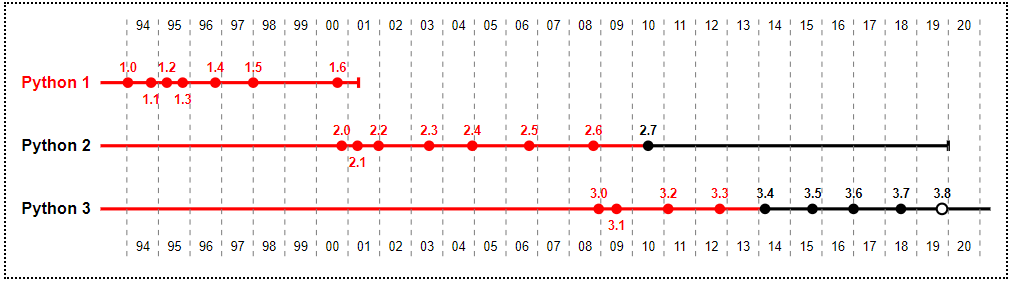
\includegraphics[width=\textwidth]{unnamed (7).png}

La imagen siguiente muestra la fecha de publicación de las últimas versiones menores de Python. Las versiones indicadas en rojo se consideran obsoletas, las versiones indicadas con punto blanco corresponden a versiones futuras con fechas ya previstas.

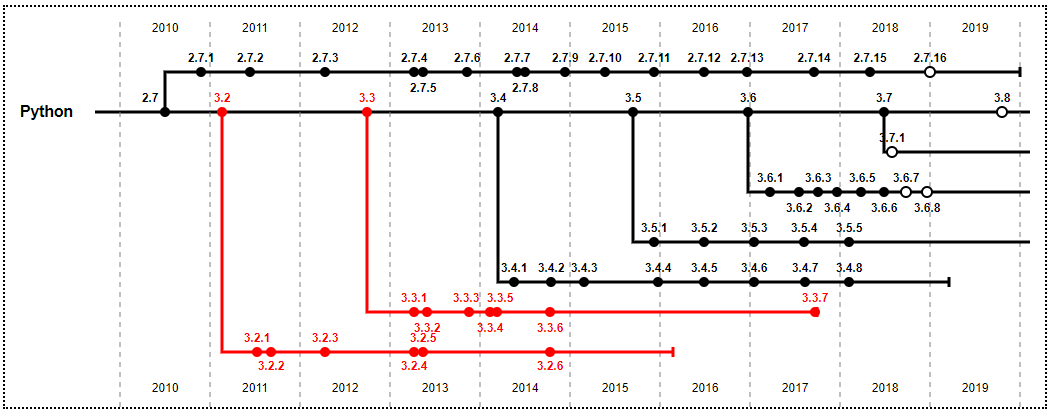
\includegraphics[width=\textwidth]{unnamed (8).png}

Es posible tener instalados en el ordenador varias versiones de Python pero, salvo que sea necesario para la ejecución de programas o paquetes incompatibles, se recomienda instalar siempre la última versión disponible.
Referencias
Principales novedades en Python (documentación oficial):
Python 2.X: 2.0 - 2.1 - 2.2 - 2.3 - 2.4 - 2.5 - 2.6 - 2.7
Python 3.X: 3.0 - 3.1 - 3.2 - 3.3 - 3.4 - 3.5 - 3.6 - 3.7
Planificación de la publicación de cada versión (release schedules):
Python 2.X: 2.6 - 2.7 - 2.8
Python 3.X: 3.0 - 3.1 - 3.2 - 3.3 - 3.4 - 3.5 - 3.6 - 3.7 - 3.8
Sobre los cambios en Python 3 (Nick Coghlan)
Cool New Features in Python 3.7, de Geir Arne Hjelle (27/06/18)
Transición de Python 2 a Python 3
La transición de Python 2 a Python 3 ha resultado mucho más costosa de lo esperado, debido a que Python 3 introdujo muchos cambios en el lenguaje y obligaba a reescribir prácticamente todos los programas (aunque se han creado herramientas para ayudar en ese proceso).
La intención inicial era haber terminado Python 2 con la versión 2.6, pero en 2010 se tuvo que publicar la versión 2.7, incorporando parte de las novedades de Python 3. Además, el período de mantenimiento de Python 2.7 se tuvo que duplicar de los cinco años habituales a diez, hasta 2020.

Un primer obstáculo en el proceso de transición de Python 2 a Python 3 ha sido la propia disponibilidad de Python 3 en las distribuciones GNU/Linux. Muchas herramientas internas de las distribuciones están escritas en Python y su conversión de Python 2 a Python 3 no era fácil, por lo que las distribuciones no podían pasar simplemente de incluir una versión a otra.
Hasta 2015, Python 2 siguió siendo la versión predeterminada de Python en la mayoría de distribuciones GNU/Linux (aunque se podía instalar Python 3 sin problemas en ellas). Felizmente, esta situación está en vías de solución:
Fedora hizo la transición a Python 3.4 en Fedora 23 (publicada en noviembre de 2015) [wiki de Fedora]. Eso quiere decir que RedHat Linux 8 (sin fecha de publicación prevista) usará Python 3. Posteriormente, Fedora 24 (publicada en junio de 2016) incluyó Python 3.5 y Fedora 26 (publicada en julio de 2017) incluyó Python 3.6.
Ubuntu hizo la transición a Python 3.5 en Ubuntu 16.04 (publicada en abril de 2016) [wiki de Ubuntu] e incluye Python 3.6 en Ubuntu 18.04 (publicada en abril de 2018) [wiki de Ubuntu].
En abril de 2015 Debian empezó a discutir los planes de transición a Python 3. Debian 9 (publicado en junio de 2017) incluye Python 2.7.13 y Python 3.5.3 y Debian 10 (que se espera publicar en 2019) debería pasar completamente a Python 3 [artículo de Linux Week News del 29/04/15].
OpenStack, una importante plataforma de virtualización, incluyó soporte para Python 3 (concretamente, Python 3.5) en la versión Pike, publicada en agosto de 2017
Aunque las nuevas versiones de las distribuciones ya incluyan Python 3, las distribuciones que incluyen Python 2 seguirán instaladas en servidores durante bastantes años. Ese es el motivo por el que se vayan a seguir publicando actualizaciones de seguridad de Python 2.7 hasta 2020, como mínimo.

Un segundo obstáculo en el proceso de transición de Python 2 a Python 3 (y que ha afectado además a todos los sistemas operativos) ha sido la disponibilidad de las bibliotecas.
Python cuenta con un gran número de bibliotecas, cuyo repositorio oficial es PyPI (Python Package Index), que facilitan la programación de aplicaciones complejas. Cuando se publicó Python 3, la inmensa mayoría de bibliotecas sólo estaban disponibles para Python 2 y, lógicamente, si un programa necesitaba alguna biblioteca que sólo estaba disponible para Python 2, el programa no se podía pasar tampoco a Python 3.
Poco a poco, la mayoría de bibliotecas de Python han ido publicando versiones para Python 3, por lo que este problema también está en vías de solución.
En marzo de 2016, un estudio de empleados de Microsoft señalaba que por aquel entonces algo más del 50\% de las bibliotecas estaban disponibles tanto para Python 2 como para Python 3, un 25\% estaban disponibles sólo para Python 2 y un poco menos del 25\% estaban disponibles sólo para Python 3, pero la tendencia parecía indicar que a mediados de 2016 Python 3 pasaría a ser la versión más popular.
Varias páginas web hacen un seguimiento de la compatibilidad con Python 3 de las bibliotecas más populares
Python 3 Wall of Superpowers (parece que desde abril de 2018 esta web ya no actualiza los datos) y Python 3 Readiness muestran cómo la inmensa mayoría de las bibliotecas más populares ya están disponibles en Python 3
la distribución GNU/Linux Fedora lleva el seguimiento de los paquetes de Python que forman parte de la distribución: paquetes y evolución.
Drop Python muestra las bibliotecas más populares han dejado de dar soporte a las versiones obsoletas de Python (Python 2.6, Python 3.2 y Python 3.3). \cite{BartolomeWebSite}


\section{La biblioteca OpenCV.}

OpenCV (Open Source Computer Vision Library) se lanza bajo licencia BSD y, por lo tanto, es gratuito tanto para uso académico como comercial. Tiene interfaces C ++, Python y Java y es compatible con Windows, Linux, Mac OS, iOS y Android. OpenCV fue diseñado para la eficiencia computacional y con un fuerte enfoque en aplicaciones en tiempo real. Escrito en C / C ++ optimizado, la biblioteca puede aprovechar el procesamiento de múltiples núcleos. Habilitado con OpenCL, puede aprovechar la aceleración de hardware de la plataforma informática heterogénea subyacente.

Adoptado en todo el mundo, OpenCV tiene más de 47 mil personas de usuarios y una cantidad estimada de descargas que supera los 14 millones. El uso va desde el arte interactivo hasta la inspección de minas, la costura de mapas en la web o la robótica avanzada. \cite{OpenCVWebSite}


OpenCV, es una biblioteca informática de código abierto desarrollado originalmente por la visión de Intel . Es gratuito para uso comercial y la investigación bajo un licencia BSD. La biblioteca es multiplataforma y funciona en Mac OSX, Windows y Linux. Se centra principalmente hacia procesamiento imagen tiempo real como tal si encuentra Intel Integrated Performance Primitives sobre el sistema, utilizará estas rutinas optimizado comerciales a acelerarse.
Diseño del proyecto

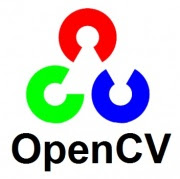
\includegraphics[width=\textwidth]{unnamed (9).jpg}

OpenCV.

Lanzado oficialmente en 1999, el proyecto fue inicialmente OpenCV iniciativa de investigación del Intel para avanzar en la CPU aplicaciones de uso intensivo, que forma parte de una serie de proyectos, entre ellos en tiempo real el trazado de rayos y las paredes de visualización 3D. Los principales contribuyentes al proyecto incluye equipo de Intel la biblioteca de rendimiento. En los primeros días de OpenCV, los objetivos del proyecto se describe como:
Avanzar en la investigación, proporcionando la visión no sólo libre, sino también el código optimizado para las infraestructuras básicas de la visión.
Difundir el conocimiento de la visión de aportar una infraestructura común que los desarrolladores pueden construir, para que el código sería más fácil lectura e intransferible.
Promover la visión basada en aplicaciones comerciales, haciendo portátiles, rendimiento optimizado de código disponible de forma gratuita con una licencia que no requiere ser abierto o gratuitas.

Historia.

Desde que apareció su primera versión alfa en el mes de enero de 1999, se ha utilizado en infinidad de aplicaciones. Desde sistemas de seguridad con detección de movimiento, hasta aplicativos de control de procesos donde se requiere reconocimiento de objetos. Esto se debe a que su publicación se da bajo licencia BSD, que permite que sea usada libremente para propósitos comerciales y de investigación con las condiciones en ella expresadas.
OpenCV es multiplataforma, existiendo versiones para GNU/Linux, Mac OSX y Windows. Contiene más de 500 funciones que abarcan una gran gama de áreas en el proceso de visión, como reconocimiento de objetos (reconocimientos facial), calibración de cámaras, visión estéreo y visión robótica.
El proyecto pretende proporcionar un entorno de desarrollo fácil de utilizar y altamente eficiente. Esto se ha logrado, realizando su programación en código C y C++ optimizados, aprovechando además las capacidades que proveen los procesadores multi núcleo. OpenCV puede además utilizar el sistema de primitivas de rendimiento integradas de Intel, un conjunto de rutinas de bajo nivel específicas para procesadores Intel (IPP).

Funciones.

Captura en tiempo real.
Importación de archivos de vídeo.
El tratamiento básico de imágenes (brillo, contraste, umbral).
Detección de objetos (cara, cuerpo).
Blob detección.

Aplicaciones.

OpenCV ha sido usado en el sistema de visión del vehículo no tripulado Stanley de la Universidad de Stanford, el ganador en el año 2005 del Gran desafío DARPA
OpenCV se usa en sistemas de vigilancia de vídeo
OpenCV es la clave en el programa Swistrack, una herramienta de seguimiento distribuida

Lenguaje de programación.

La biblioteca fue originalmente escrita en C y esta interfaz C hace OpenCV portátil para algunas plataformas específicas,tales como procesadores de señal digital.
OpenCV incluye tanto la interfaz de C tradicionales, así como una nueva interfaz C++, que busca reducir el número de líneas de código necesarias al código de la funcionalidad de la visión, así como reducir los errores comunes de programación, tales como la memoria fugas que pueden surgir al utilizar OpenCV en la mayoría de los nuevos desarrollos y algoritmos OpenCV C.
Se desarrollan en el interfaz C++, es mucho más difícil para las envolturas en otras lenguas de código C++ en lugar de código en C. \cite{SourgeForgeWebSite} \cite{UbaaWebSite} \cite{YahooWebSite}

\end{document}